\documentclass{ximera}
\graphicspath{  %% When looking for images,
{./}            %% look here first,
{./pictures/}   %% then look for a pictures folder,
{../pictures/}  %% which may be a directory up.
{../../pictures/}  %% which may be a directory up.
{../../../pictures/}  %% which may be a directory up.
{../../../../pictures/}  %% which may be a directory up.
}

\usepackage{listings}
%\usepackage{circuitikz}
\usepackage{xcolor}
\usepackage{amsmath,amsthm}
\usepackage{subcaption}
\usepackage{graphicx}
\usepackage{tikz}
%\usepackage{tikz-3dplot}
\usepackage{amsfonts}
%\usepackage{mdframed} % For framing content
%\usepackage{tikz-cd}

  \renewcommand{\vector}[1]{\left\langle #1\right\rangle}
  \newcommand{\arrowvec}[1]{{\overset{\rightharpoonup}{#1}}}
  \newcommand{\ro}{\texttt{R}}%% row operation
  \newcommand{\dotp}{\bullet}%% dot product
  \renewcommand{\l}{\ell}
  \let\defaultAnswerFormat\answerFormatBoxed
  \usetikzlibrary{calc,bending}
  \tikzset{>=stealth}
  




%make a maroon color
\definecolor{maroon}{RGB}{128,0,0}
%make a dark blue color
\definecolor{darkblue}{RGB}{0,0,139}
%define the color fourier0 to be the maroon color
\definecolor{fourier0}{RGB}{128,0,0}
%define the color fourier1 to be the dark blue color
\definecolor{fourier1}{RGB}{0,0,139}
%define the color fourier 1t to be the light blue color
\definecolor{fourier1t}{RGB}{173,216,230}
%define the color fourier2 to be the dark green color
\definecolor{fourier2}{RGB}{0,100,0}
%define teh color fourier2t to be the light green color
\definecolor{fourier2t}{RGB}{144,238,144}
%define the color fourier3 to be the dark purple color
\definecolor{fourier3}{RGB}{128,0,128}
%define the color fourier3t to be the light purple color
\definecolor{fourier3t}{RGB}{221,160,221}
%define the color fourier0t to be the red color
\definecolor{fourier0t}{RGB}{255,0,0}
%define the color fourier4 to be the orange color
\definecolor{fourier4}{RGB}{255,165,0}
%define the color fourier4t to be the darker orange color
\definecolor{fourier4t}{RGB}{255,215,0}
%define the color fourier5 to be the yellow color
\definecolor{fourier5}{RGB}{255,255,0}
%define the color fourier5t to be the darker yellow color
\definecolor{fourier5t}{RGB}{255,255,100}
%define the color fourier6 to be the green color
\definecolor{fourier6}{RGB}{0,128,0}
%define the color fourier6t to be the darker green color
\definecolor{fourier6t}{RGB}{0,255,0}

%New commands for this doc for errors in copying
\newcommand{\eigenvar}{\lambda}
%\newcommand{\vect}[1]{\mathbf{#1}}
\renewcommand{\th}{^{\text{th}}}
\newcommand{\st}{^{\text{st}}}
\newcommand{\nd}{^{\text{nd}}}
\newcommand{\rd}{^{\text{rd}}}
\newcommand{\paren}[1]{\left(#1\right)}
\newcommand{\abs}[1]{\left|#1\right|}
\newcommand{\R}{\mathbb{R}}
\newcommand{\C}{\mathbb{C}}
\newcommand{\Hilb}{\mathbb{H}}
\newcommand{\qq}[1]{\text{#1}}
\newcommand{\Z}{\mathbb{Z}}
\newcommand{\N}{\mathbb{N}}
\newcommand{\q}[1]{\text{``#1''}}
%\newcommand{\mat}[1]{\begin{bmatrix}#1\end{bmatrix}}
\newcommand{\rref}{\text{reduced row echelon form}}
\newcommand{\ef}{\text{echelon form}}
\newcommand{\ohm}{\Omega}
\newcommand{\volt}{\text{V}}
\newcommand{\amp}{\text{A}}
\newcommand{\Seq}{\textbf{Seq}}
\newcommand{\Poly}{\textbf{P}}
\renewcommand{\quad}{\text{    }}
\newcommand{\roweq}{\simeq}
\newcommand{\rowop}{\simeq}
\newcommand{\rowswap}{\leftrightarrow}
\newcommand{\Mat}{\textbf{M}}
\newcommand{\Func}{\textbf{Func}}
\newcommand{\Hw}{\textbf{Hamming weight}}
\newcommand{\Hd}{\textbf{Hamming distance}}
\newcommand{\rank}{\text{rank}}
\newcommand{\longvect}[1]{\overrightarrow{#1}}
% Define the circled command
\newcommand{\circled}[1]{%
  \tikz[baseline=(char.base)]{
    \node[shape=circle,draw,inner sep=2pt,red,fill=red!20,text=black] (char) {#1};}%
}

% Define custom command \strikeh that just puts red text on the 2nd argument
\newcommand{\strikeh}[2]{\textcolor{red}{#2}}

% Define custom command \strikev that just puts red text on the 2nd argument
\newcommand{\strikev}[2]{\textcolor{red}{#2}}

%more new commands for this doc for errors in copying
\newcommand{\SI}{\text{SI}}
\newcommand{\kg}{\text{kg}}
\newcommand{\m}{\text{m}}
\newcommand{\s}{\text{s}}
\newcommand{\norm}[1]{\left\|#1\right\|}
\newcommand{\col}{\text{col}}
\newcommand{\sspan}{\text{span}}
\newcommand{\proj}{\text{proj}}
\newcommand{\set}[1]{\left\{#1\right\}}
\newcommand{\degC}{^\circ\text{C}}
\newcommand{\centroid}[1]{\overline{#1}}
\newcommand{\dotprod}{\boldsymbol{\cdot}}
%\newcommand{\coord}[1]{\begin{bmatrix}#1\end{bmatrix}}
\newcommand{\iprod}[1]{\langle #1 \rangle}
\newcommand{\adjoint}{^{*}}
\newcommand{\conjugate}[1]{\overline{#1}}
\newcommand{\eigenvarA}{\lambda}
\newcommand{\eigenvarB}{\mu}
\newcommand{\orth}{\perp}
\newcommand{\bigbracket}[1]{\left[#1\right]}
\newcommand{\textiff}{\text{ if and only if }}
\newcommand{\adj}{\text{adj}}
\newcommand{\ijth}{\emph{ij}^\text{th}}
\newcommand{\minor}[2]{M_{#2}}
\newcommand{\cofactor}{\text{C}}
\newcommand{\shift}{\textbf{shift}}
\newcommand{\startmat}[1]{
  \left[\begin{array}{#1}
}
\newcommand{\stopmat}{\end{array}\right]}
%a command to give a name to explorations and hints and theorems
\newcommand{\name}[1]{\begin{centering}\textbf{#1}\end{centering}}
\newcommand{\vect}[1]{\vec{#1}}
\newcommand{\dfn}[1]{\textbf{#1}}
\newcommand{\transpose}{\mathsf{T}}
\newcommand{\mtlb}[2][black]{\texttt{\textcolor{#1}{#2}}}
\newcommand{\RR}{\mathbb{R}} % Real numbers
\newcommand{\id}{\text{id}}
\newcommand{\coord}[1]{\langle#1\rangle}
\newcommand{\RREF}{\text{RREF}}
\newcommand{\Null}{\text{Null}}
\newcommand{\Nullity}{\text{Nullity}}
\newcommand{\Rank}{\text{Rank}}
\newcommand{\Col}{\text{Col}}
\newcommand{\Ef}{\text{EF}}
\newcommand{\boxprod}[3]{\abs{(#1\times#2)\cdot#3}}

\author{Zack Reed}
%borrowed from selinger linear algebra
\title{Singular Value Decomposition (SVD)}
\begin{document}
\begin{abstract}

\end{abstract}
\maketitle

\section*{Introduction: Matrix Decompositions}
In previous sections we've spent much time multiplying matrices together to form single matrices representing the emalgumation of the transformations from each matrix in the product. 

For instance, the matrix $A=\begin{bmatrix} 2 & -1 \\ 3 & 0\end{bmatrix}$ is the product of a $90^\circ$ rotation matrix $\begin{bmatrix}0 & -1\\ 1 & 0\end{bmatrix}$, a shear $\begin{bmatrix} 1 & 2 \\ 0 & 1\end{bmatrix}$ and a vertical stretch $\begin{bmatrix} 1 & 0 \\ 0 & 3\end{bmatrix}$. We're cheating a little bit since we know how $A$ was built, but we could say that $A$ can be \emph{decomposed} into three matrices via the product 

$$\begin{bmatrix} 2 & -1 \\ 3 & 0\end{bmatrix}=\begin{bmatrix} 1 & 0 \\ 0 & 3\end{bmatrix}*\begin{bmatrix} 1 & 2 \\ 0 & 1\end{bmatrix}*\begin{bmatrix}0 & -1\\ 1 & 0\end{bmatrix}.$$

You can check this effect by transforming points by the matrix $A$, such as the points in $\texttt{+linalg/face\_points.mat}$ via

\begin{verbatim}

  load +linalg/face_points.mat
  rotate_1=[cos(pi/2) -sin(pi/2);
    sin(pi/2) cos(pi/2)]
  shear_1=[1 2;
      0 1]
  stretch_y=[1 0;
      0 3]
  A=stretch_y*shear_1*rotate_1
  trans_face=A*face_points
  linalg.simple_plot_cloud(trans_face);

\end{verbatim}

which yields the following figure 

%1120x840
\begin{center}
  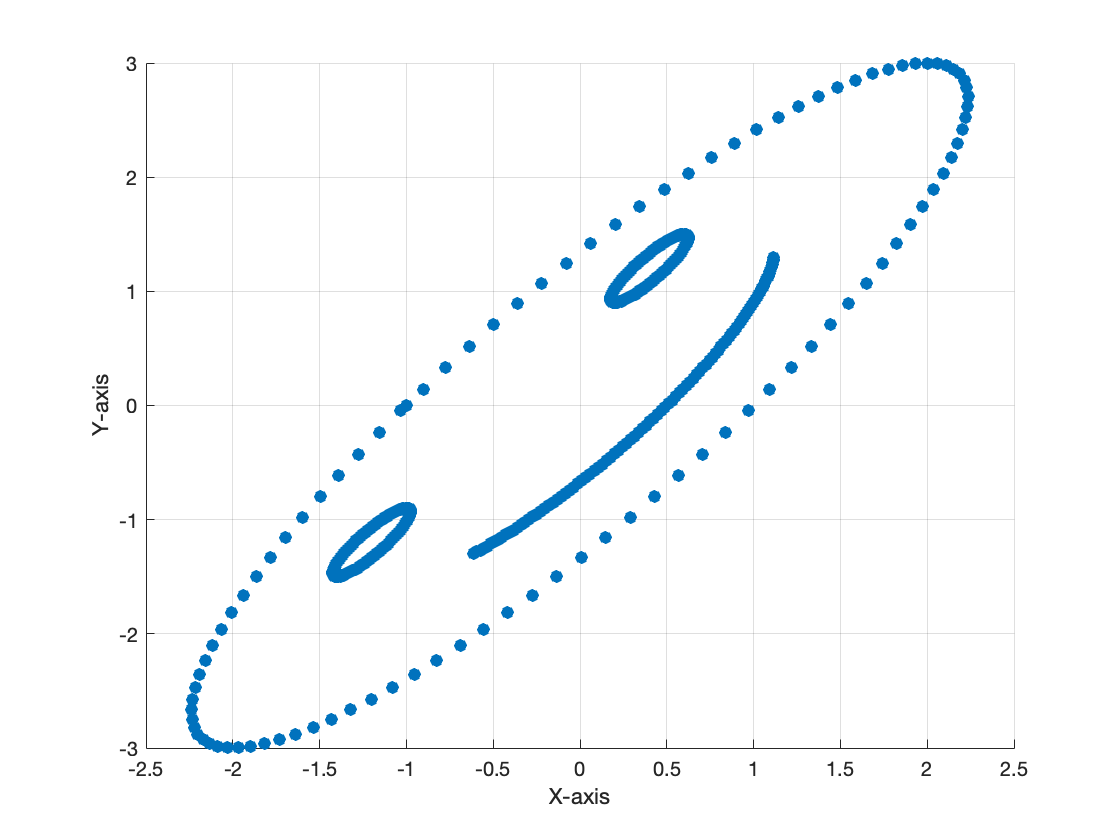
\includegraphics[width=29.63cm, height=22.22cm]{face_svd_intro_A.png}
\end{center}

If you then individually apply the transformations to $\texttt{face\_points}$, you should yeild the same figure. 

We also spent a considerable amount of time finding inverse matrices as products of elementary matrices via Gaussian Elimination. For instance, if we reverse the transformations (i.e. find the inverse of each transformation) we then get the inverse matrix $A^{-1}$.

Reversing a vertical stretch is the vertical compression $\begin{bmatrix}1 &0\\
  0 &1/3\end{bmatrix}$ which yields

  \begin{verbatim}

    reverse_face=[1 0;0 1/3]*trans_face
    linalg.simple_plot_cloud(reverse_face)

  \end{verbatim}

  %1120x840
\begin{center}
  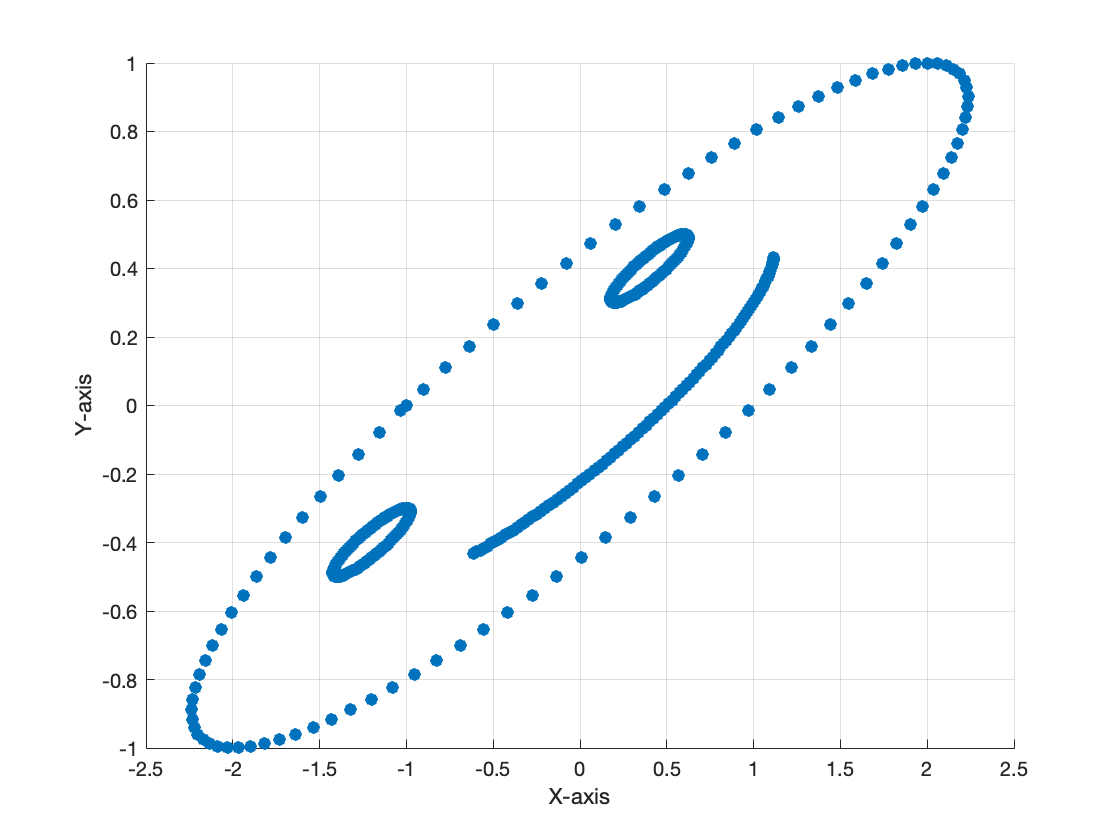
\includegraphics[width=29.63cm, height=22.22cm]{face_svd_intro_A_reverse_1.png}
\end{center}

then you un-do the shear by shearing in the reverse direction $\begin{bmatrix}1 &-2\\
  0 &1\end{bmatrix}$ which yields 

  \begin{verbatim}

    reverse_face=[1 -2;0 1]*reverse_face
    linalg.simple_plot_cloud(reverse_face)

  \end{verbatim}

  %1120x840
\begin{center}
  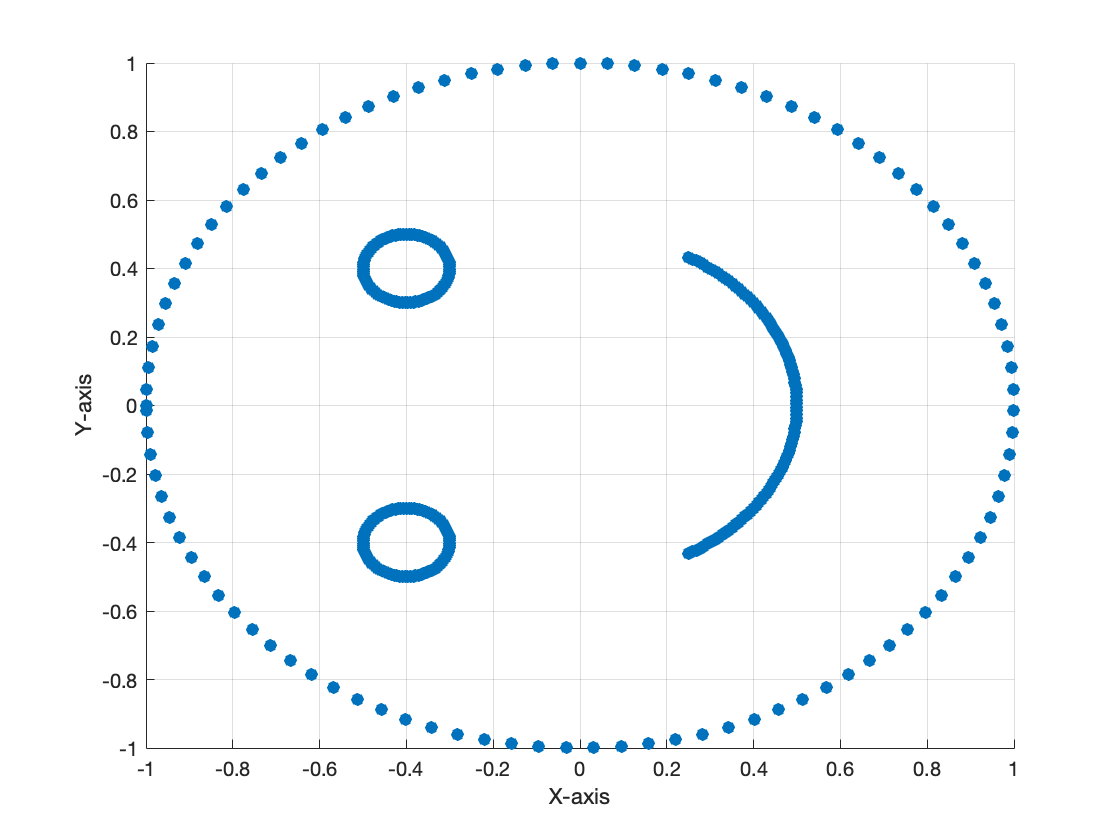
\includegraphics[width=29.63cm, height=22.22cm]{face_svd_intro_A_reverse_2.png}
\end{center}

and then you un-do the rotation by rotating in the reverse direction $\begin{bmatrix}\cos(-\pi/2) & -\sin(-\pi/2)\\
  \sin(-\pi/2) & \cos(-\pi/2)\end{bmatrix}$,

  \begin{verbatim}

    reverse_face=[0 -1;-1 0]*reverse_face
    linalg.simple_plot_cloud(reverse_face)

  \end{verbatim}

which yields the original face.

This means that we have a decomposition of $A^{-1}$ as 
$$\begin{bmatrix}\cos(-\pi/2) & -\sin(-\pi/2)\\\sin(-\pi/2) & \cos(-\pi/2)\end{bmatrix}*\begin{bmatrix}1 &-2\\0 &1\end{bmatrix}*\begin{bmatrix}1 &0\\0 &1/3\end{bmatrix}=\begin{bmatrix}0 & 1/3\\-1 & 2/3\end{bmatrix}.$$

Important data analysis techniques arising from Linear Algebra recreate this process of \emph{decomposition}, but start with a matrix for which we don't know the decomposition and end with the product of two or more matrices that make up the matrix. This would be akin to starting with $A$, performing some Linear Algebra manipulations on $A$, and ending up with the otherwise unknown matrices $\begin{bmatrix} 1 & 0 \\ 0 & 3\end{bmatrix}$, $\begin{bmatrix} 1 & 2 \\ 0 & 1\end{bmatrix}$, and $\begin{bmatrix}0 & -1\\ 1 & 0\end{bmatrix}$. 


The analysis on voting records in \href{https://ximera.osu.edu/appliedlinearalgebra/c6ChapterSix/learningActivities/m6LearningActivities/leastSquares/leastSquaresApplicationVotingImages}{the previous section} can be performed through a special matrix decomposition called the \emph{singular value decomposition}. This particular decomposition forms the backbone of many modern data analysis techniques, and is at times the first step one takes when buildling machine learlning models today. The \emph{singular value decomposition} (SVD) is also useful in engineering, the sciences, and many software-based applications. We will be using the SVD as a context in which to unpack many important ideas in Linear Algebra.

n many mathematics texts, you spend the majority of your time learning how to \emph{compute} something, often by hand, and then only later do you learn \emph{why} you might make a computation or \emph{how} a computation can be used for various tasks. Hopefully this process accompanies some intuition about why the computation works the way it does. 

As you move beyond this course, however, and especially once you progress into your specific domains of study (engineering, data science, etc.), you will increasingly rely on technology to perform computations for you and your primary job is to know \emph{when} to make a computation, to \emph{interpret} the result of that computation, and to know \emph{what went wrong or right} when a computation yielded an unexpected result. 

We will foreground this latter approach to learning the SVD. In many respects, we have already been employing these emphases already, but this focus will be especially true for the SVD as we will gain a general understanding of one method of SVD computation at the very end of this chapter, and then gain other more employable computations in later chapters, but will largely spend our time: learning \emph{what} the SVD is, learning \emph{how} to use it in various situations, and using technology to calculate it for us.

\section{SVD Part 1: Rotations and Stretches}

The first important aspect of the SVD is that it decomposes \emph{any} matrix $M$ into three matrices, often called $U$, $S$, and $V$ (though you can label these matrices whatever you want). This is a very important utility of the SVD, that it works on any matrix. Many other useful decompositions only work on certain matrices with special conditions.

Let's explore the properties of these $U$, $S$, and $V$ matrices by re-examining our original matrix $A=\begin{bmatrix} 2 & -1 \\ 3 & 0\end{bmatrix}$.

To find the SVD in MATLAB, use the syntax $\texttt{[U, S, V]=svd(A)}$. $\texttt{svd()}$ is one of those functions that gives multiple outputs, so if you don't list and name each output it will only return the first output (in this case the $U$ matrix). (Note: Sometimes you'll see $V$ denoted as $V^\dagger$ and $S$ denoted as $\Sigma$ we will just use $S$ and $V$)

The decomposition is that $A=U*S*V^{T}$. 

\begin{problem}
Use MATLAB to explore the properties of $U, S$, and $V$ below, selecting all that are true. Use $\texttt{face\_points}$ as a test subject for the transformations associated with $U$, $S$, and $V$.

\begin{selectAll}

  \choice[correct]{$V$ is a rotation matrix.}
  \choice{$U$ represents a shear transformation.}
  \choice[correct]{$S$ is a diagonal matrix.}
  \choice{$S$ swaps the coordinate axes.}
  \choice[correct]{The columns of $U$ are all unit vectors.}
  \choice{$U$ maps vectors into the null space of $A$.}
  \choice{$V$ maps vectors into the column space of $A$.}
  \choice{$V$ translates the rows of $A$ to a new origin.}
  \choice[correct]{$U$ is a rotation matrix.}
  \choice{$U$ scales the columns of $A$ by the diagonal of $S$ values.}
  \choice{$V$ is an upper triangular matrix.}
  \choice[correct]{The columns of $V$ are all unit vectors.}
  \choice[correct]{$S$ stretches and compresses along the coordinate axes.}
  \choice{$S$ represents a projection onto the row space of $A$.}
  \choice{$U$ permutes the rows of $A$.}
  \choice{$U*S*V$ also equals $A$.}
  \choice{$V$ flips the sign of all elements in $A$.}

\end{selectAll}

\begin{feedback}

  Let's explore the transformational interpretations of the SVD first. In short, the SVD lets you write any matrix as the product of \emph{two rotations} and a \emph{stretching}. This is much simpler than breaking down a matrix into elementary transformations, and even will work on matrices representing many transformations.

  Trying this out on our $A$ matrix, we get $V^T=\begin{bmatrix}
    -.9871 & .1602 \\ .1602 & .9871
  \end{bmatrix}$. If we apply this to \facepoints with

  \begin{verbatim}
    new_face=V'*face_points
    linalg.simple_plot_cloud(new_face);
  \end{verbatim}

  we get the image

    %1120x840
    \begin{center}
      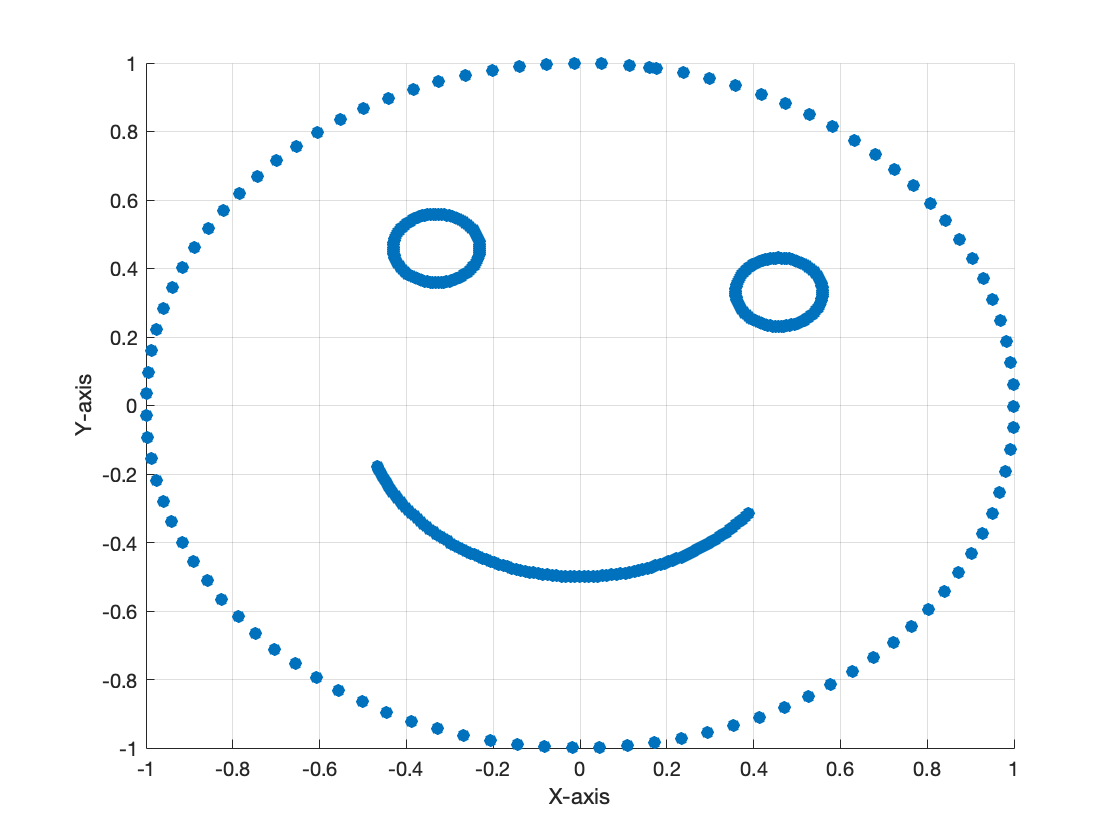
\includegraphics[width=29.63cm, height=22.22cm]{face_svd_rots_V_A.png}
    \end{center}

  Notice that this is a rotation of \facepoints, but a different rotation than the construction rotation from the introduction.
  
  If we then apply $S$ to $V^T*face\_points$, we get 

  \begin{verbatim}
    new_face=S*new_face
    linalg.simple_plot_cloud(new_face);
  \end{verbatim}

  we get the image

    %1120x840
    \begin{center}
      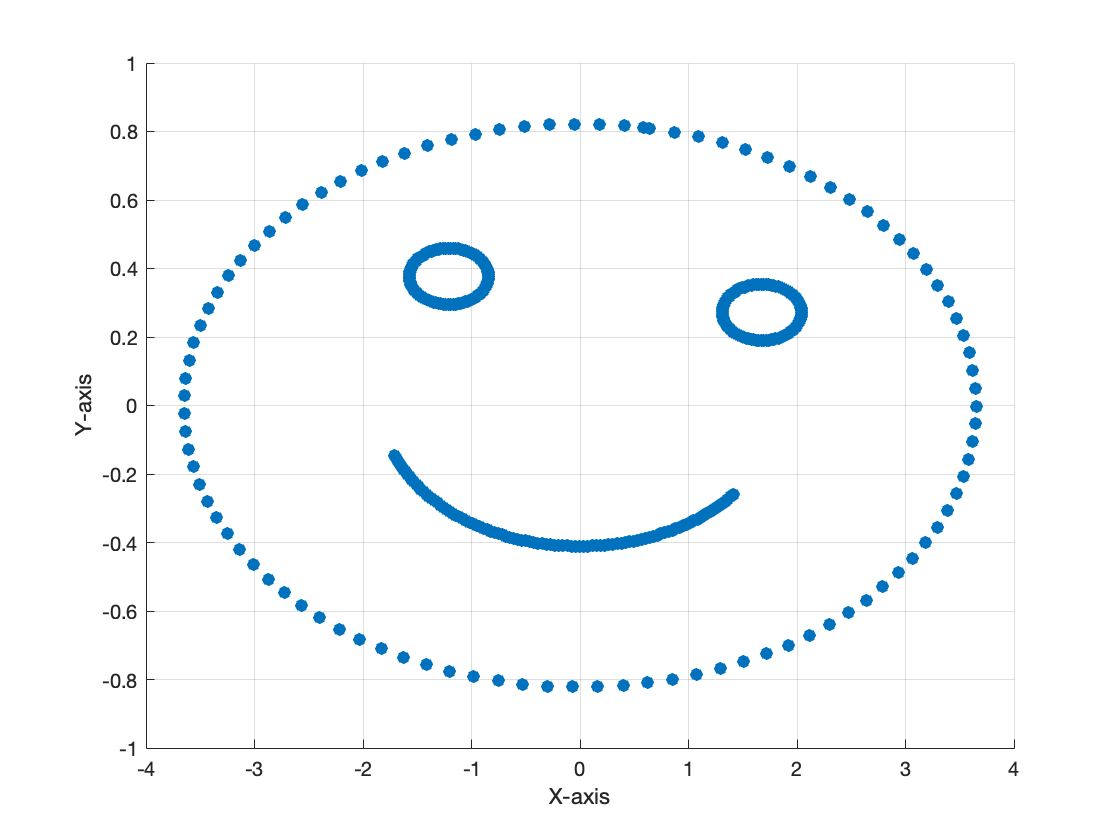
\includegraphics[width=29.63cm, height=22.22cm]{face_svd_rots_S_A.png}
    \end{center}

  Checking the dimensions of the new figure window, we notice that the face has compressed vertically inward and stretched horizontally outward, according to the diagonal values of $S$.

  Finally, if we apply $U$ to $S*V'*face\_points$, we get 

  \begin{verbatim}
    new_face=U*new_face
    linalg.simple_plot_cloud(new_face);
  \end{verbatim}

  we get the same figure as when we apply $A$ to \facepoints. 

  Keeping in mind the dimensions of the face image after multiplication by $S$, you'll note that $U$ applied another rotation. 

  Finally, with a couple of quick for loops you'll note that teh columns of both $U$ and $V$ are unit vectors. 

\end{feedback}

\end{[problem]}

As we said before, the SVD can be applied to \emph{any} matrix, unlike many decompositions that require square matrices. Let's again explore the SVD, but on two nonsquare matrices that map $3$-dimensional vectors.

We'll first examine a rank 2 3x3 matrix, and then a 3x2 matrix, as these both will illuminate some important structural aspects of the SVD matrices. 

First, consider $B=\begin{bmatrix}1&3&-3\\0&1&-2\\1&-3&9\end{bmatrix}$. A quick use of $\texttt{rref(B)}$ or $\texttt{rank(B)}$ indeed confirms the rank of 2. 

We can further note the rank of $B$ by observing its effect on a $3$D cloud of vectors, say $\texttt{+linalg/smiley\_3D.mat}$. 

\begin{verbatim}

  B=[1 0 1;
  3 1 -3]
  load +linalg/smiley_3D.mat
  linalg.simple_plot_cloud(head, eyes, smile);
  face=[head,eyes,smile]
  two_face=B*face
  linalg.simple_plot_cloud(two_face);
\end{verbatim}

which yeilds the plots 

%1120x840
\begin{center}
  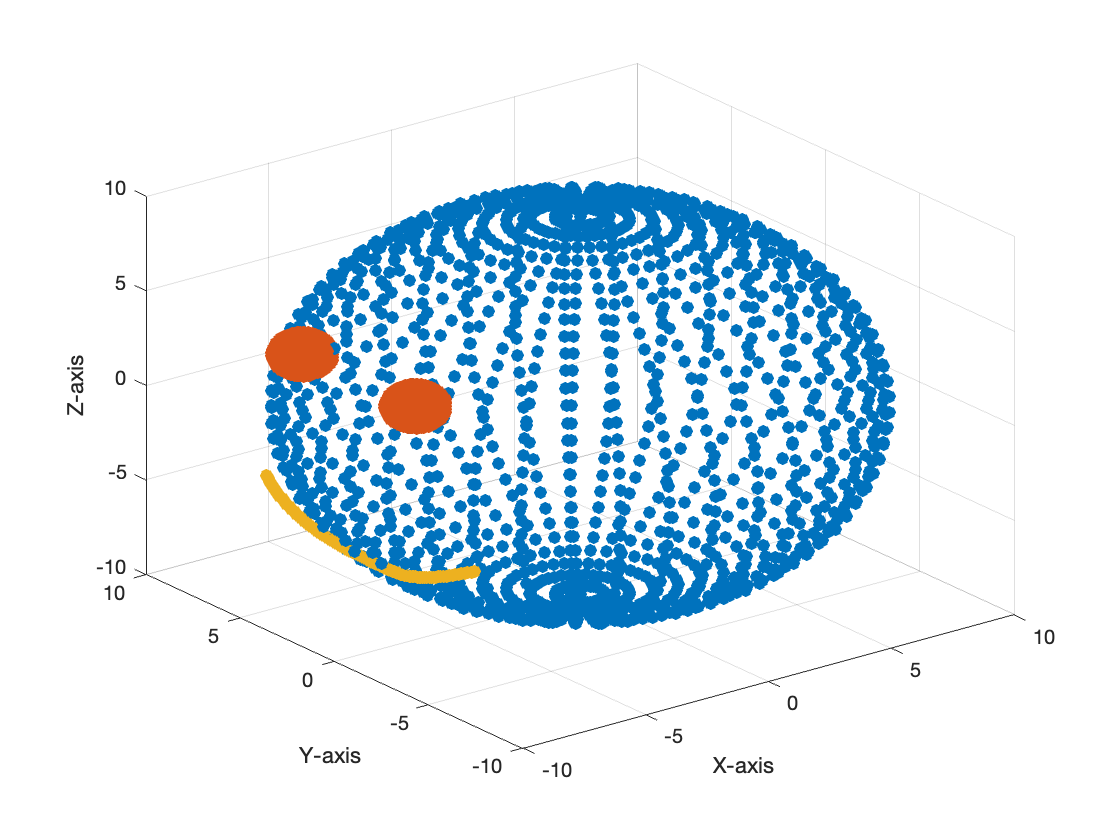
\includegraphics[width=29.63cm, height=22.22cm]{face_svd_3D.png}
\end{center}

    and 

%1120x840
\begin{center}
  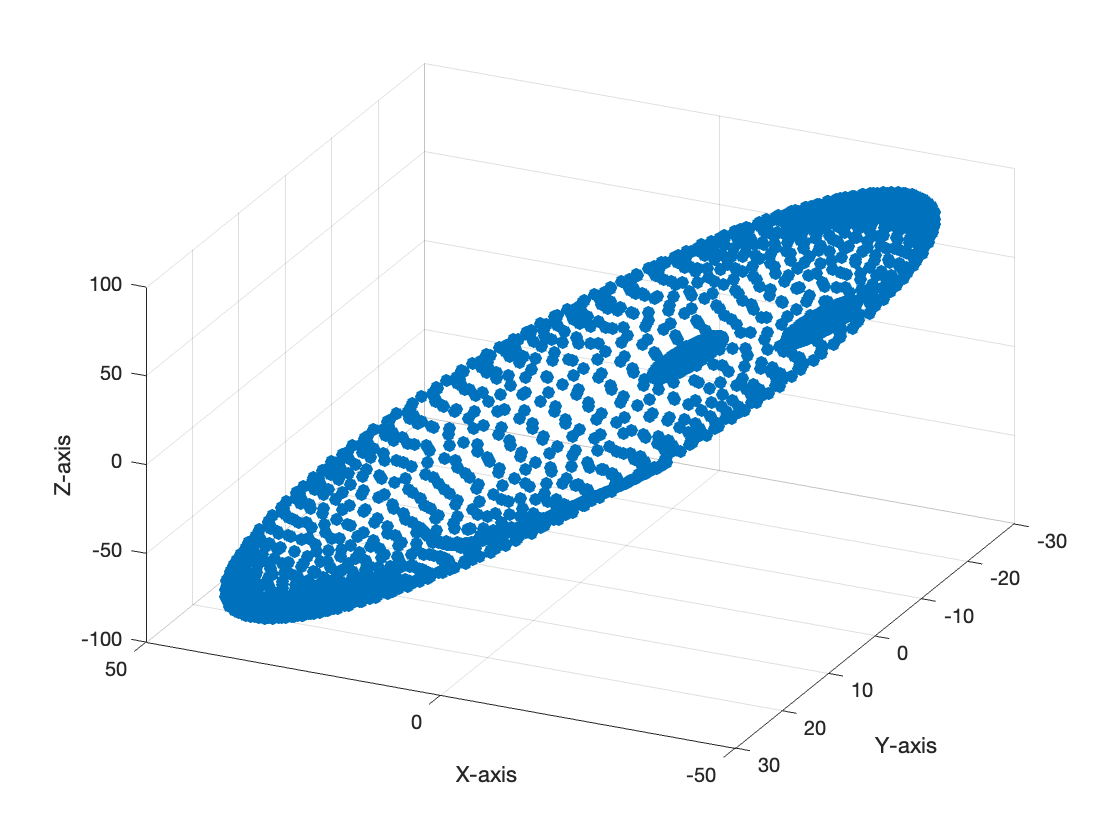
\includegraphics[width=29.63cm, height=22.22cm]{face_svd_3D_B_2D.png}
\end{center}

This visualizes more specifically the structure of $B$ in that it compresses space down to a plane. While further analysis of $B$ can determine which vectors span the image space, we can actually determine this same information from the SVD. 

First, remember that the SVD breaks down any matrix into two rotations and a stretch. Let's see these in action.

After taking the SVD, we start with the matrix $V_B^T$.

\begin{verbatim}

  [U_B, S_B, V_B]=svd(B)
  two_face=V_B'*face
  linalg.simple_plot_cloud(two_face)

\end{verbatim}

which yields

%1120x840
\begin{center}
  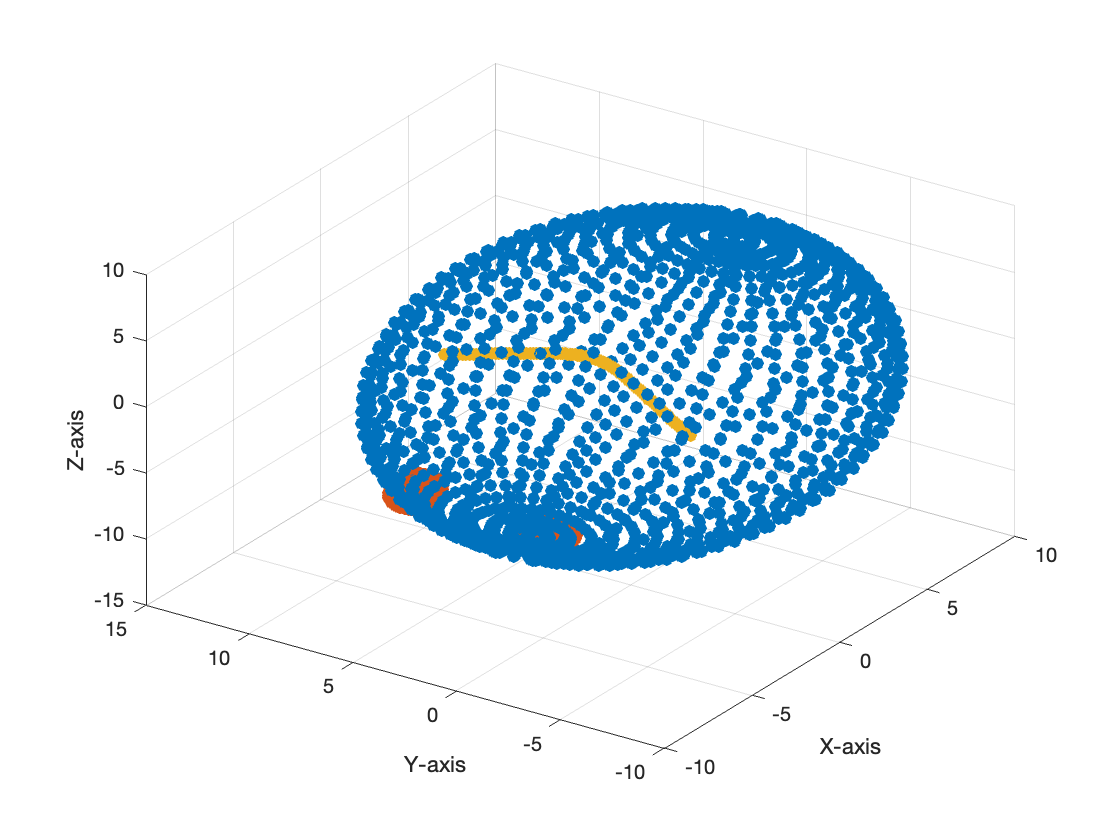
\includegraphics[width=29.63cm, height=22.22cm]{face_svd_3D_B_V.png}
\end{center}

(Note: I maintained the head, eyes, and smile separately for these figures so that the rotations were more evident.). This clearly performed a rotation in space.

Then, we follow up by multiplying by $S_B$.

\begin{verbatim}

  two_face=S_B*two_face
  linalg.simple_plot_cloud(two_face)

\end{verbatim}

which yields

%1120x840
\begin{center}
  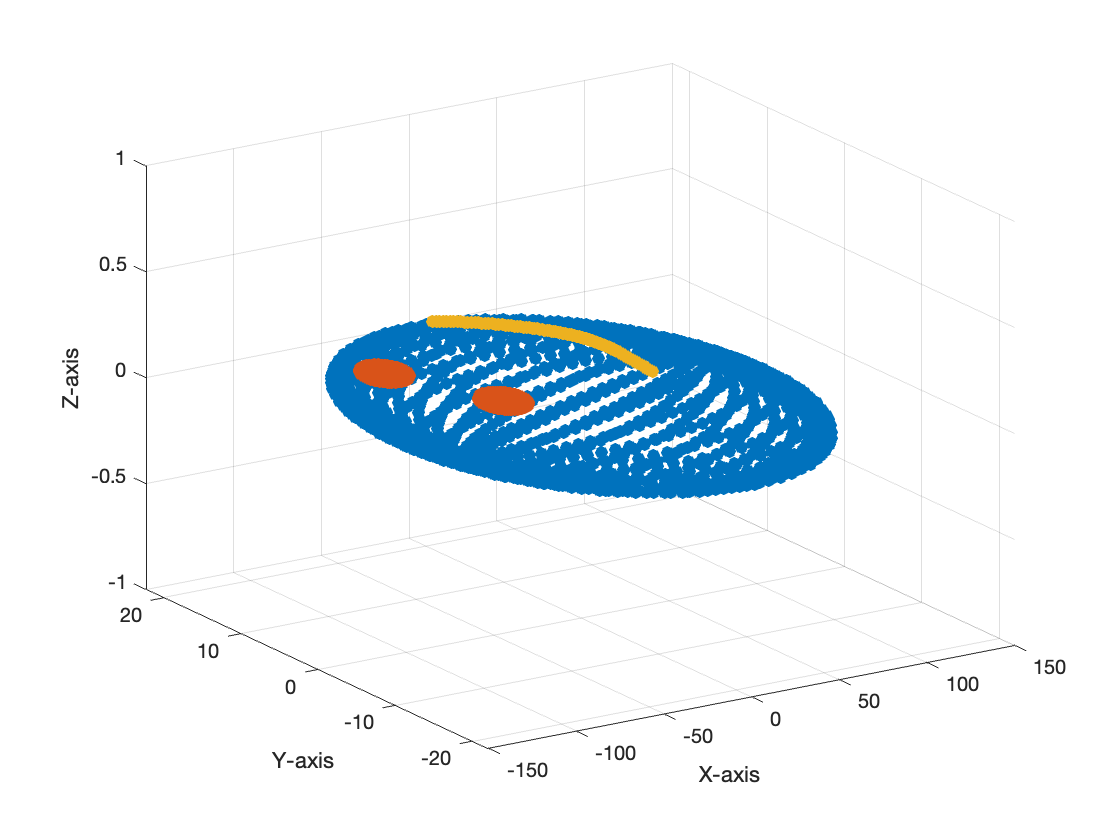
\includegraphics[width=29.63cm, height=22.22cm]{face_svd_3D_B_S.png}
\end{center}

Note that this time, the cloud flattened into a $2D$ disc. Then, we finish by multiplying by $U_B$.

\begin{verbatim}

  two_face=U_B*two_face
  linalg.simple_plot_cloud(two_face)

\end{verbatim}

which yields

%1120x840
\begin{center}
  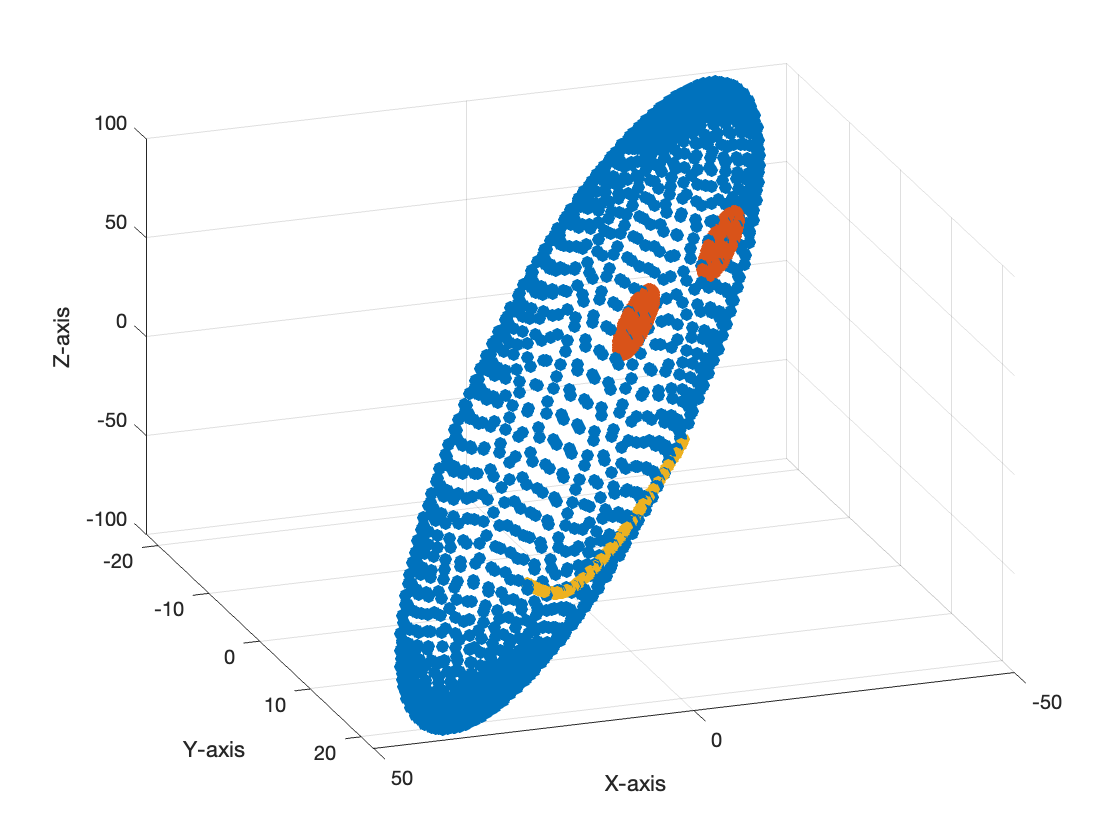
\includegraphics[width=29.63cm, height=22.22cm]{face_svd_3D_B_U.png}
\end{center}

Once again, we have a rotation applied to the disc, and this final transformation matches the result of multiplication by $B$.

What you might notice from this third figure is that the flattened disc is not round and circular, but actually quite stretched in two directions. If you inspect the axes more closely after multiplication by $S_B$, you'll note that this stretching was indeed present, as the $x,y,z$ axes spanned $[-100,100]$, $[-20,20]$ and $[-1,1]$.

\begin{problem}

Based on this analysis, mark which statement is correct about the SVD in this example.

\begin{multipleChoice}

  \choice{$U$ controlled the rank of $B$}
  \choice[correct]{$S$ controlled the rank of $B$}
  \choice{$V$ controlled the rank of $B$}

\end{multipleChoice}

\begin{feedback}

  In fact, you can explain the rank of $B$ by the compressing stage of multiplication by $S$. Since $S$ is diagonal, it stretched and compressed the rotated face matrix along the standard axes. The $x$-direction got stretched by around $10$, the $y$-direction got stretched by around $2$, but the $z$-direction flattened, resulting in a $2$-dimensional disc which was then rotated by $U$. You can in fact describe the process of constructing $B$ from the SVD as: 

  \begin{enumerate}
    \item $V^T$ rotates space to set up stretching and compression by $S$
    \item $S$ stretches and compresses space according to the rank (and amount of spread) of the matrix (more on this later).
    \item $U$ rotates the stretched and compressed space to the directions over which $B$ spreads image vectors.
  \end{enumerate}

\end{feedback}

We can actually be even more specific, beyond merely saying $U$ and $V$ rotate and $S$ compresses. There is in fact important and specific information gained by the columns of $U$ and $V$, as well as the diagonal elements of $S$. 

We will adopt specific terminology to refer to these vectors and values. The columns of $U$ are the \emph{left singular vectors}, the columns of $V$ are the \emph{right singular vectors}, and the diagonal values of $S$ are the \emph{singular values} of a matrix $M$. You can for now distinguish the left and right singular vectors by the order of multiplication $U*S*V^T$.

If you plot the columns of $U$ (the left singular vectors) alongside the final transformation (after scaling for visibility), you get the following 

%1120x840
\begin{center}
  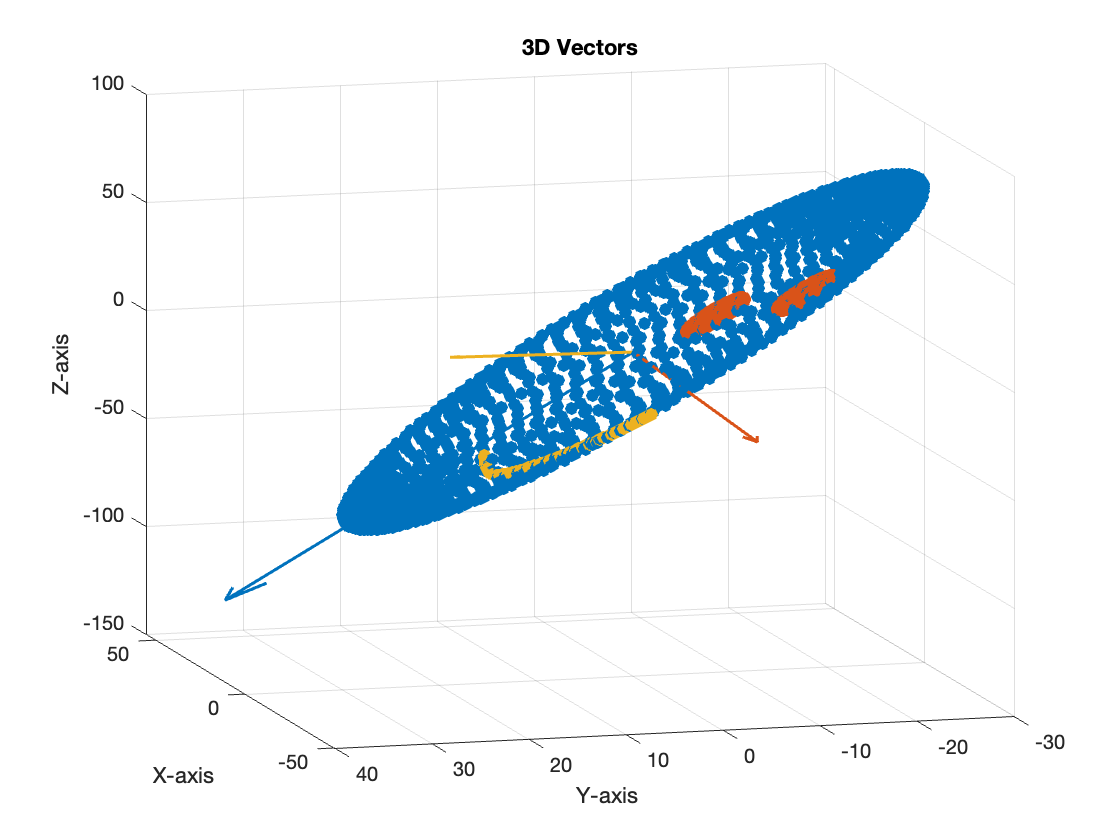
\includegraphics[width=29.63cm, height=22.22cm]{face_svd_B_U_vects.png}
\end{center}

\begin{hint}\name{MATLAB Code}
  \begin{verbatim}

    linalg.simple_plot_cloud(two_head,two_eyes,two_smile);
    hold on
    linalg.simple_plot_quiver(150*U_B(:,1),50*U_B(:,2),20*U_B(:,3));
    hold off
  
  \end{verbatim}
\end{hint}

The blue vector is the first singular vector, the red is the second, and the yellow is the third. If you plot this yourself and rotate the figure, you'll note that the first two singular vectors orthogonally span the plane on which the disc sits (and hence span the image of the transformation), and the third singular vector is perpendicular to the plane. 

Even more important, the first singular vector points in the direction of the maximum stretching of the disc, the second points in the next direction of stretching, and the third points away from the disc, where there is no stretching. If you return to the singular values (the diagonal of $S$), you actually get a direct correspondance of the amount of stretching (which makes sense, since $S$ stretches and compresses the sphere after rotation by $V$). So the sphere was first stretched by a factor of $10$ (the first singular value) in the $x$-direction, then by a factor of $2$ (the second singular vector) in the $y$-direction, and then by a factor of $0$ (the third singular vector) in the $z$-direction. 

The left singular vectors then rotated space so that the $10$-stretched axis pointed in the direction of $u_1=\begin{bmatrix}.3684\\.2123\\-.9051\end{bmatrix}$, the $2$-stretched axis pointed in the direction of $u_2=\begin{bmatrix}-.9154\\-.0871\\-.3930\end{bmatrix}$, and then the final singular vector points in the direction over the remaining 


\section{SVD}
Any matrix \(A\) can be factorized as:

\[
A = U \Sigma V^\top
\]

where \(U\) and \(V\) are orthogonal matrices and \(\Sigma\) is a diagonal matrix with elements equal to the square root of the positive eigenvalues of \(AA^\top\) or \(A^\top A\).

\[
A = U \begin{bmatrix} \sigma_1 & 0 & \cdots \\ 0 & \sigma_2 & \cdots \\ \vdots & \vdots & \ddots \end{bmatrix} V^\top
\]

The columns of \(U\) are called the left singular vectors, and those of \(V\) are the right singular vectors.

\section{Example}
Consider an example of a simple \(2 \times 2\) matrix. We calculate:

\[
A = \begin{bmatrix} 3 & 1 \\ 1 & 3 \end{bmatrix}
\]

The singular values are \(\sigma_1 = 5\) and \(\sigma_2 = 3\). Thus, the SVD composition is:

\[
A = U \Sigma V^\top
\]

\section{Recap of SVD}
The SVD decomposition of \(A\) can be summarized as:

\[
A = U \Sigma V^\top
\]

where

\[
U^\top U = I \quad \text{and} \quad V^\top V = I
\]

\section{Moore-Penrose Pseudoinverse}
To find the best-fit solution, we compute a pseudoinverse of \(A\) that minimizes the least square error:

\[
A^+ = V \Sigma^+ U^\top
\]

\section{Variance \& Covariance}
The sample variance is defined as:

\[
s^2 = \frac{1}{n-1} \sum_{i=1}^n (x_i - \bar{x})^2
\]

The covariance matrix \(\Sigma\) captures variance along the diagonal elements and covariance between variables in the non-diagonal elements.

\section{Covariance Matrix \& SVD}
The SVD decomposition of a covariance matrix reveals the principal components of data. The total variance of the data equals the trace of the covariance matrix, which is the sum of the squares of singular values.

\section{Principal Component Analysis (PCA)}
Technically, SVD extracts data in the directions with the highest variances. PCA uses SVD for mapping data to principal components, allowing dimensionality reduction by ignoring less significant terms.

One of the early and natural ideas in software development for scientific computation was the idea of packaging linear algebra software around robust implementations of matrix factorizations, divested from specific applications. This enabled durable linear algebra tools like LAPACK to be developed with a stable interface, usable across numerous application domains. Commercial software like Matlab™, as well as open-source software like Octave, numpy, and scipy, all take full advantage of these developments. What does this mean for you as an aspiring data scientist? When you are faced with a specific computational task, if you are able to reformulate your task using off-the-shelf implementations of matrix factorizations, then you might already be halfway to finishing your task.

You already know about some matrix factorizations. In your introductory linear algebra prerequisites, you learned about eigenvalues and eigenvectors. The computation of eigenvalues and eigenvectors is indeed the computation of a matrix factorization. This factorization is called a diagonalization or an eigenvalue decomposition of an \( n \times n \) matrix \( A \) and it takes the form

\[
A = X D X^{-1}
\]

where \( D \) is a diagonal matrix and \( X \) is an invertible matrix, both of the same size as \( A \). The eigenvalues of \( A \) are found in the diagonal entries of \( D \) and the eigenvectors are columns of \( X \), as can be seen by rewriting the factorization as

\[
A X = X D.
\]

The importance of eigenvalues in varied applications is usually highlighted well in a first linear algebra course.

Another important factorization is the SVD, or the singular value decomposition, which often does not get the emphasis it deserves in lower-division courses. In some ways, the SVD is even more important than diagonalization. This is because not all matrices have a diagonalization. In contrast, using basic real analysis results, one can prove that any matrix has an SVD. We shall see that from an SVD, one can read off the important properties of a matrix and easily construct compressed approximations of the matrix.

\section{Definition of SVD}

The SVD is a factorization of an \( m \times n \) matrix \( A \) of the form

\[
A = U \Sigma V^*
\]

where \( \Sigma \) is an \( m \times n \) diagonal matrix, and \( U \) and \( V \) are unitary matrices of size \( m \times m \) and \( n \times n \), respectively. (Recall that a square matrix \( Q \) is called unitary if its inverse equals \( Q^* \), the conjugate transpose of \( Q \).) The diagonal entries of \( \Sigma \) are non-negative, and positive ones are called the singular values of \( A \). It is a convention to list the singular values in non-increasing order along the diagonal. The columns of \( U \) and \( V \) are called the left and right singular vectors, respectively.

Here is how we compute SVD using MATLAB:

\begin{verbatim}
[U, S, V] = svd(rand(4, 5) + 1i * rand(4, 5));
U * U'  % U is unitary. Its columns are left singular vectors
V * V'  % Rows of V are right singular vectors
diag(S) % Only the diagonal entries of Sigma are returned in S
\end{verbatim}

\section{The Algebra of SVD}

An outer product of an \( x \in \mathbb{R}^m \) and \( y \in \mathbb{R}^n \) is the \( m \times n \) matrix \( x y^* \) (which, being the product of \( m \times 1 \) and \( 1 \times n \) matrices, is of shape \( m \times n \)). Reversing the order of \( x \) and \( y^* \) in the product, we get the familiar inner product, which is a \( 1 \times 1 \) matrix or a scalar.

Naming the columns of \( U \) and \( V \) as \( u_i \) and \( v_j \), we have

\[
A = U \Sigma V^* = \sum_{l=1}^{\min(m,n)} \sigma_l u_l v_l^*.
\]

Thus, the SVD can be viewed as a sum of unit-rank outer products. Each summand increases rank (if the corresponding singular value is nonzero) until the rank of \( A \) is reached. Let's see this in action for a small matrix in MATLAB.

\begin{verbatim}
a = rand(4, 5);
[U, S, V] = svd(a);
outer_product = U(:, 1) * V(1, :) * S(1, 1);
\end{verbatim}

\section{Low Rank Approximation}

A useful application of SVD is low-rank approximation. For an \( m \times n \) matrix \( A \) with singular values \( \sigma_j \), we can approximate \( A \) using the first few singular values:

\[
A_\ell = \sum_{j=1}^\ell \sigma_j u_j v_j^*.
\]

This is particularly useful for image compression. Here’s how to compute a low-rank approximation of an image using MATLAB:

\begin{verbatim}
img = imread('cats.png');
img = img(:,:,1); % Convert to grayscale
[U, S, V] = svd(double(img));
rank_20 = U(:, 1:20) * S(1:20, 1:20) * V(:, 1:20)';
imshow(uint8(rank_20), []);
\end{verbatim}

If you increase the rank, the approximation becomes closer to the original image. This technique not only reduces storage requirements but can also accelerate computations by reducing the dimensions of data.

\section{Further Applications}

The SVD is a fundamental tool for any data scientist. Whether it’s image compression, dimensionality reduction, or uncovering hidden structures in data, SVD provides a robust mathematical framework that continues to be valuable across many domains.

Returning to Theorem 2, notice that the theorem also gives one the ability to specify an error tolerance and let that dictate the choice of the rank \( \ell \). For example, if I do not want the error in my low-rank approximation to be more than some specific \( \epsilon \), then I need only choose \( \ell \) so that:

\[
\left( \sigma_{\ell+1}^2 + \cdots + \sigma_{r}^2 \right)^{1/2} \leq \epsilon.
\]

As an example, suppose I declare I want a low-rank approximation within the following relative error in Frobenius norm:

\begin{verbatim}
relative_error = 1.e-1;
\end{verbatim}

Then we can find the needed \( \ell \) using an aggregation and masking as follows:

\begin{verbatim}
s2 = s.^2;
total = sum(s2);
diff = sqrt((total - cumsum(s2)) / total);
l = find(diff < relative_error, 1);
l
\end{verbatim}

This will output:

\begin{verbatim}
l = 41
\end{verbatim}

Then, here is the needed low-rank approximation:

\begin{verbatim}
cl = U(:, 1:l) * diag(s(1:l)) * V(:, 1:l)';
\end{verbatim}

You can check that the error is indeed less than the prescribed error tolerance:

\begin{verbatim}
error = norm(c - cl, 'fro') / norm(c, 'fro');
error
\end{verbatim}

This returns:

\begin{verbatim}
error = 0.09942439
\end{verbatim}

As you can see, the low-rank approximation does give some image compression. The number of entries needed to store a rank \( \ell \) approximation \( cl \) of an \( m \times n \) matrix is \( m\ell + \ell + \ell n \):

\begin{verbatim}
entries_needed = size(U, 1) * l + l + l * size(V, 1);
entries_needed
\end{verbatim}

For instance, this might output:

\begin{verbatim}
entries_needed = 73759
\end{verbatim}

In contrast, to store the original image (single channel), we would need to minimally store \( mn \) numbers:

\begin{verbatim}
original_entries = size(c, 1) * size(c, 2);
original_entries
\end{verbatim}

Which might output:

\begin{verbatim}
original_entries = 788320
\end{verbatim}

Comparing the two outputs, we can certainly conclude that we have some compression. However, for image compression, there are better algorithms.

The utility of the low-rank approximation technique using the SVD is not really in image compression, but rather in other applications needing a condensed operator. Being a compressed approximation of an operator (i.e., a matrix) is much more than just a compressed visual image. For example, one can not only reduce the storage for a matrix but also reduce the time to apply the operator to a vector using a low-rank approximation. Because the SVD tells us the essentials of an operator in lower-dimensional spaces, it continues to find new applications in many modern emerging concepts, some of which we shall see in later lectures.
 
\begin{center}
    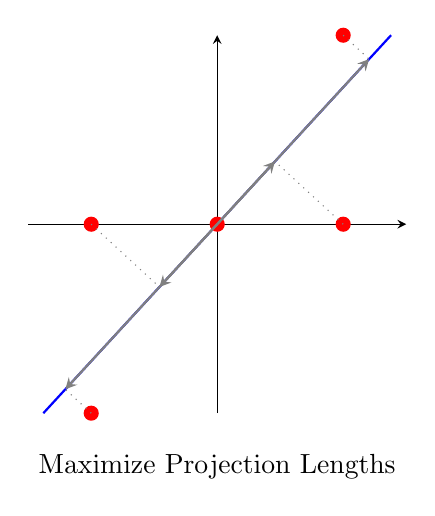
\begin{tikzpicture}[scale=0.8]
        \draw[thin,->] (-3,0) -- (3,0);
        \draw[thin,->] (0,-3) -- (0,3);
        \draw[thick,blue] (-3*0.92,-3) -- (3*0.92, 3);
        \fill[color=red] (0,0) circle (0.12);
        \fill[color=red] (2,0) circle (0.12);
        \fill[color=red] (2,3) circle (0.12);
        \fill[color=red] (-2,0) circle (0.12);
        \fill[color=red] (-2,-3) circle (0.12);
        \draw[thin, dotted,black!50] (2,0) -- (0.997*0.92,0.997);
        \draw[thin, dotted,black!50] (2,3) -- (2.621*0.92,2.621);
        \draw[thin, dotted,black!50] (-2,0) -- (-0.997*0.92,-0.997);
        \draw[thin, dotted,black!50] (-2,-3) -- (-2.621*0.92,-2.621);
        \draw[thick, ->,black!50] (0,0) -- (0.997*0.92,0.997);
        \draw[thick, ->,black!50] (0,0) -- (2.621*0.92,2.621);
        \draw[thick, ->,black!50] (0,0) -- (-0.997*0.92,-0.997);
        \draw[thick, ->,black!50] (0,0) -- (-2.621*0.92,-2.621);
        \path (0,-3.5) node[below] {Maximize Projection Lengths};
        %\path[black!70] (2,-2) node {\begin{tabular}{c}maximize\\projection\\lengths\\on subspace\end{tabular}};
      \end{tikzpicture}
    \hspace{1in}
    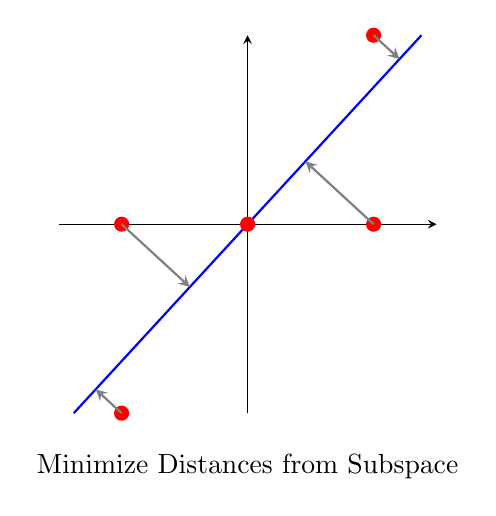
\begin{tikzpicture}[scale=0.8]
      \draw[thin,->] (-3,0) -- (3,0);
      \draw[thin,->] (0,-3) -- (0,3);
      \draw[thick,blue] (-3*0.92,-3) -- (3*0.92, 3);
      \fill[color=red] (0,0) circle (0.12);
      \fill[color=red] (2,0) circle (0.12);
      \fill[color=red] (2,3) circle (0.12);
      \fill[color=red] (-2,0) circle (0.12);
      \fill[color=red] (-2,-3) circle (0.12);
      \draw[thick, ->,black!50] (2,0) -- (0.997*0.92,0.997);
      \draw[thick, ->,black!50] (2,3) -- (2.621*0.92,2.621);
      \draw[thick, ->,black!50] (-2,0) -- (-0.997*0.92,-0.997);
      \draw[thick, ->,black!50] (-2,-3) -- (-2.621*0.92,-2.621);
      \path (0,-3.5) node[below] {Minimize Distances from Subspace};
      %\path[black!70] (2,-2) node {\begin{tabular}{c}minimize\\distances\\perpendicular\\to subspace\end{tabular}};
    \end{tikzpicture}
  \end{center}

  \begin{center}
    \geogebra{hp7wxjegkk}{630}{631}
  \end{center}


\end{document}